\chapter{Results and analysis}\label{chapter:res-analysis}
The objective of this section is to show the effect of running the test benchmarks under SPM's watch. To this end the main indicators to watch are the completion time and throughput. The first part of this chapter deals with the presentations of the results for distgen and LAMA-CG and the second part presents a discussion of these results.
 
\section{SPM and distgen}\label{section:spmydistgen}
This section will discuss the different scenarios that will be used for the testing of distgen as the observed process. For an overview of distgen, please refer to section \ref{section:distgen}.
\subsection{SPM and distgen with two threads}\label{subsection:res-spmydistgen-2t}

\subsubsection{Scenarios under consideration}\label{subsection:res-scenarios-2t-scens}

\begin{itemize}
	\item The \textbf{vanilla local scenario} is the code in its original form, two threads are run in the same NUMA node.
	\item The \textbf{vanilla remote scenario}: Each thread runs on a separate NUMA node. The first thread initializes the memory space and the second thread accesses it. 
	\item The \textbf{SPM scenario} is the same as the vanilla remote scenario but this time the program execution will be overseen by the SPM tool and the pages observed to be accessed more from a remote node are moved to the node that originates the greater number of memory accesses.
	\item The \textbf{moveall} scenario is a distgen modification based on vanilla remote that after a determinate time of execution will move all the memory pages from a remote node to a local node.
\end{itemize}

Every one of this scenarios has a specific significance for the measurement of the performance: The vanilla local scenario shows the maximum speed possible for the given algorithm, vanilla remote will show how much performance deteriorates when the algorithm is forced to perform many remote accesses in order to fetch the required data, moveall is a reference scenario that tells how much it is possible to fix the performance degradation by taking the pages placed in a remote node and bringing them close to the executing node and SPM also tries to fix the slowdown caused by the remote placement of the pages, but since the SPM does not know about the internal implementation of the supervised process, it will only move the pages that the PMU reports as remote accesses. The closer SPM's results are to the moveall scenario, the best performing the SPM tool is. Figures \ref{fig:dgentt-local} and \ref{fig:dgentt-remote} present depictions of both local and remote vanilla scenarios.

In order to be able to be able to place the pages remotely, a modification has to be made to the original distgen code, where the initialization is done by the master thread and the access is done only by the other thread, which is not the master. To determine whether the two threads are placed in a local node the environment variable \textit{GOMP\_CPU\_AFFINITY} is manipulated in order to determine the core in which the running threads will be placed. The availability of this modified two threads version is described in code listing 5 in Appendix \ref{app:coderes}.

\begin{figure}
	\centering
		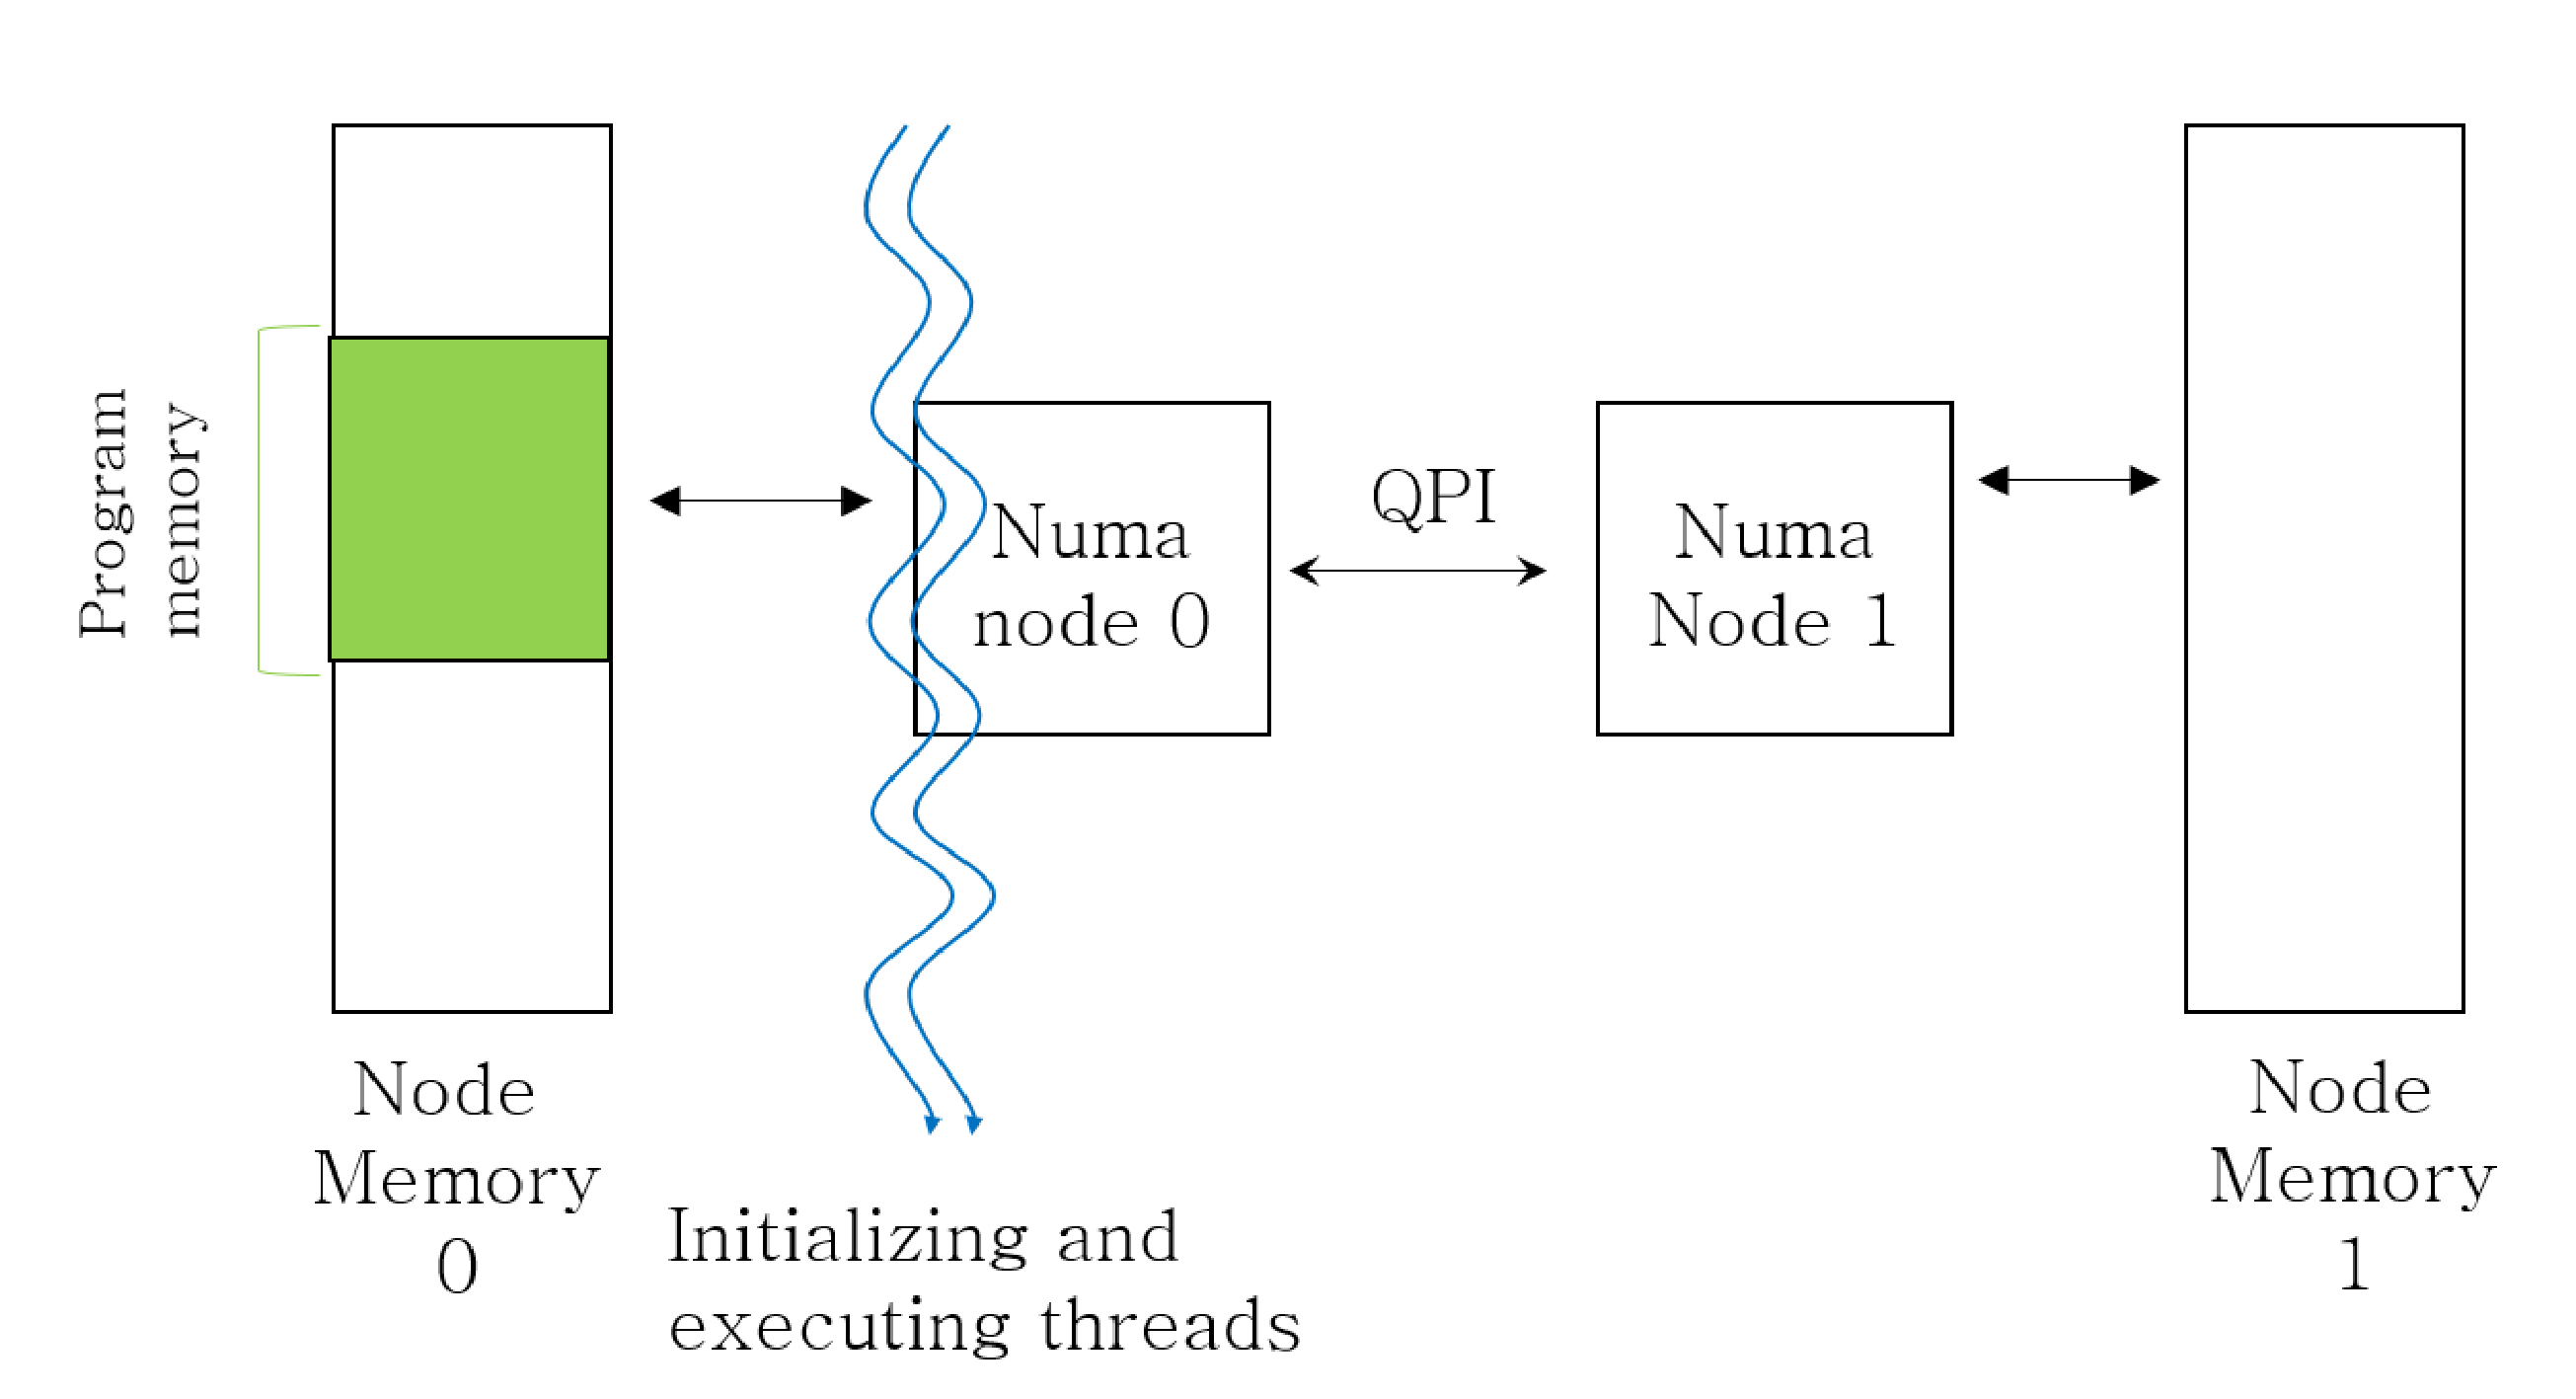
\includegraphics[width=.7\textwidth]{figures/distgentt-local.eps}
		\caption[Depiction of the working of the distgen vanilla local scenario with two threads]{Depiction of the distgen vanilla local with two running threads. Both threads are in the same NUMA node, therefore only local accesses will be performed.}
		\label{fig:dgentt-local}
\end{figure}

\begin{figure}
	\centering
		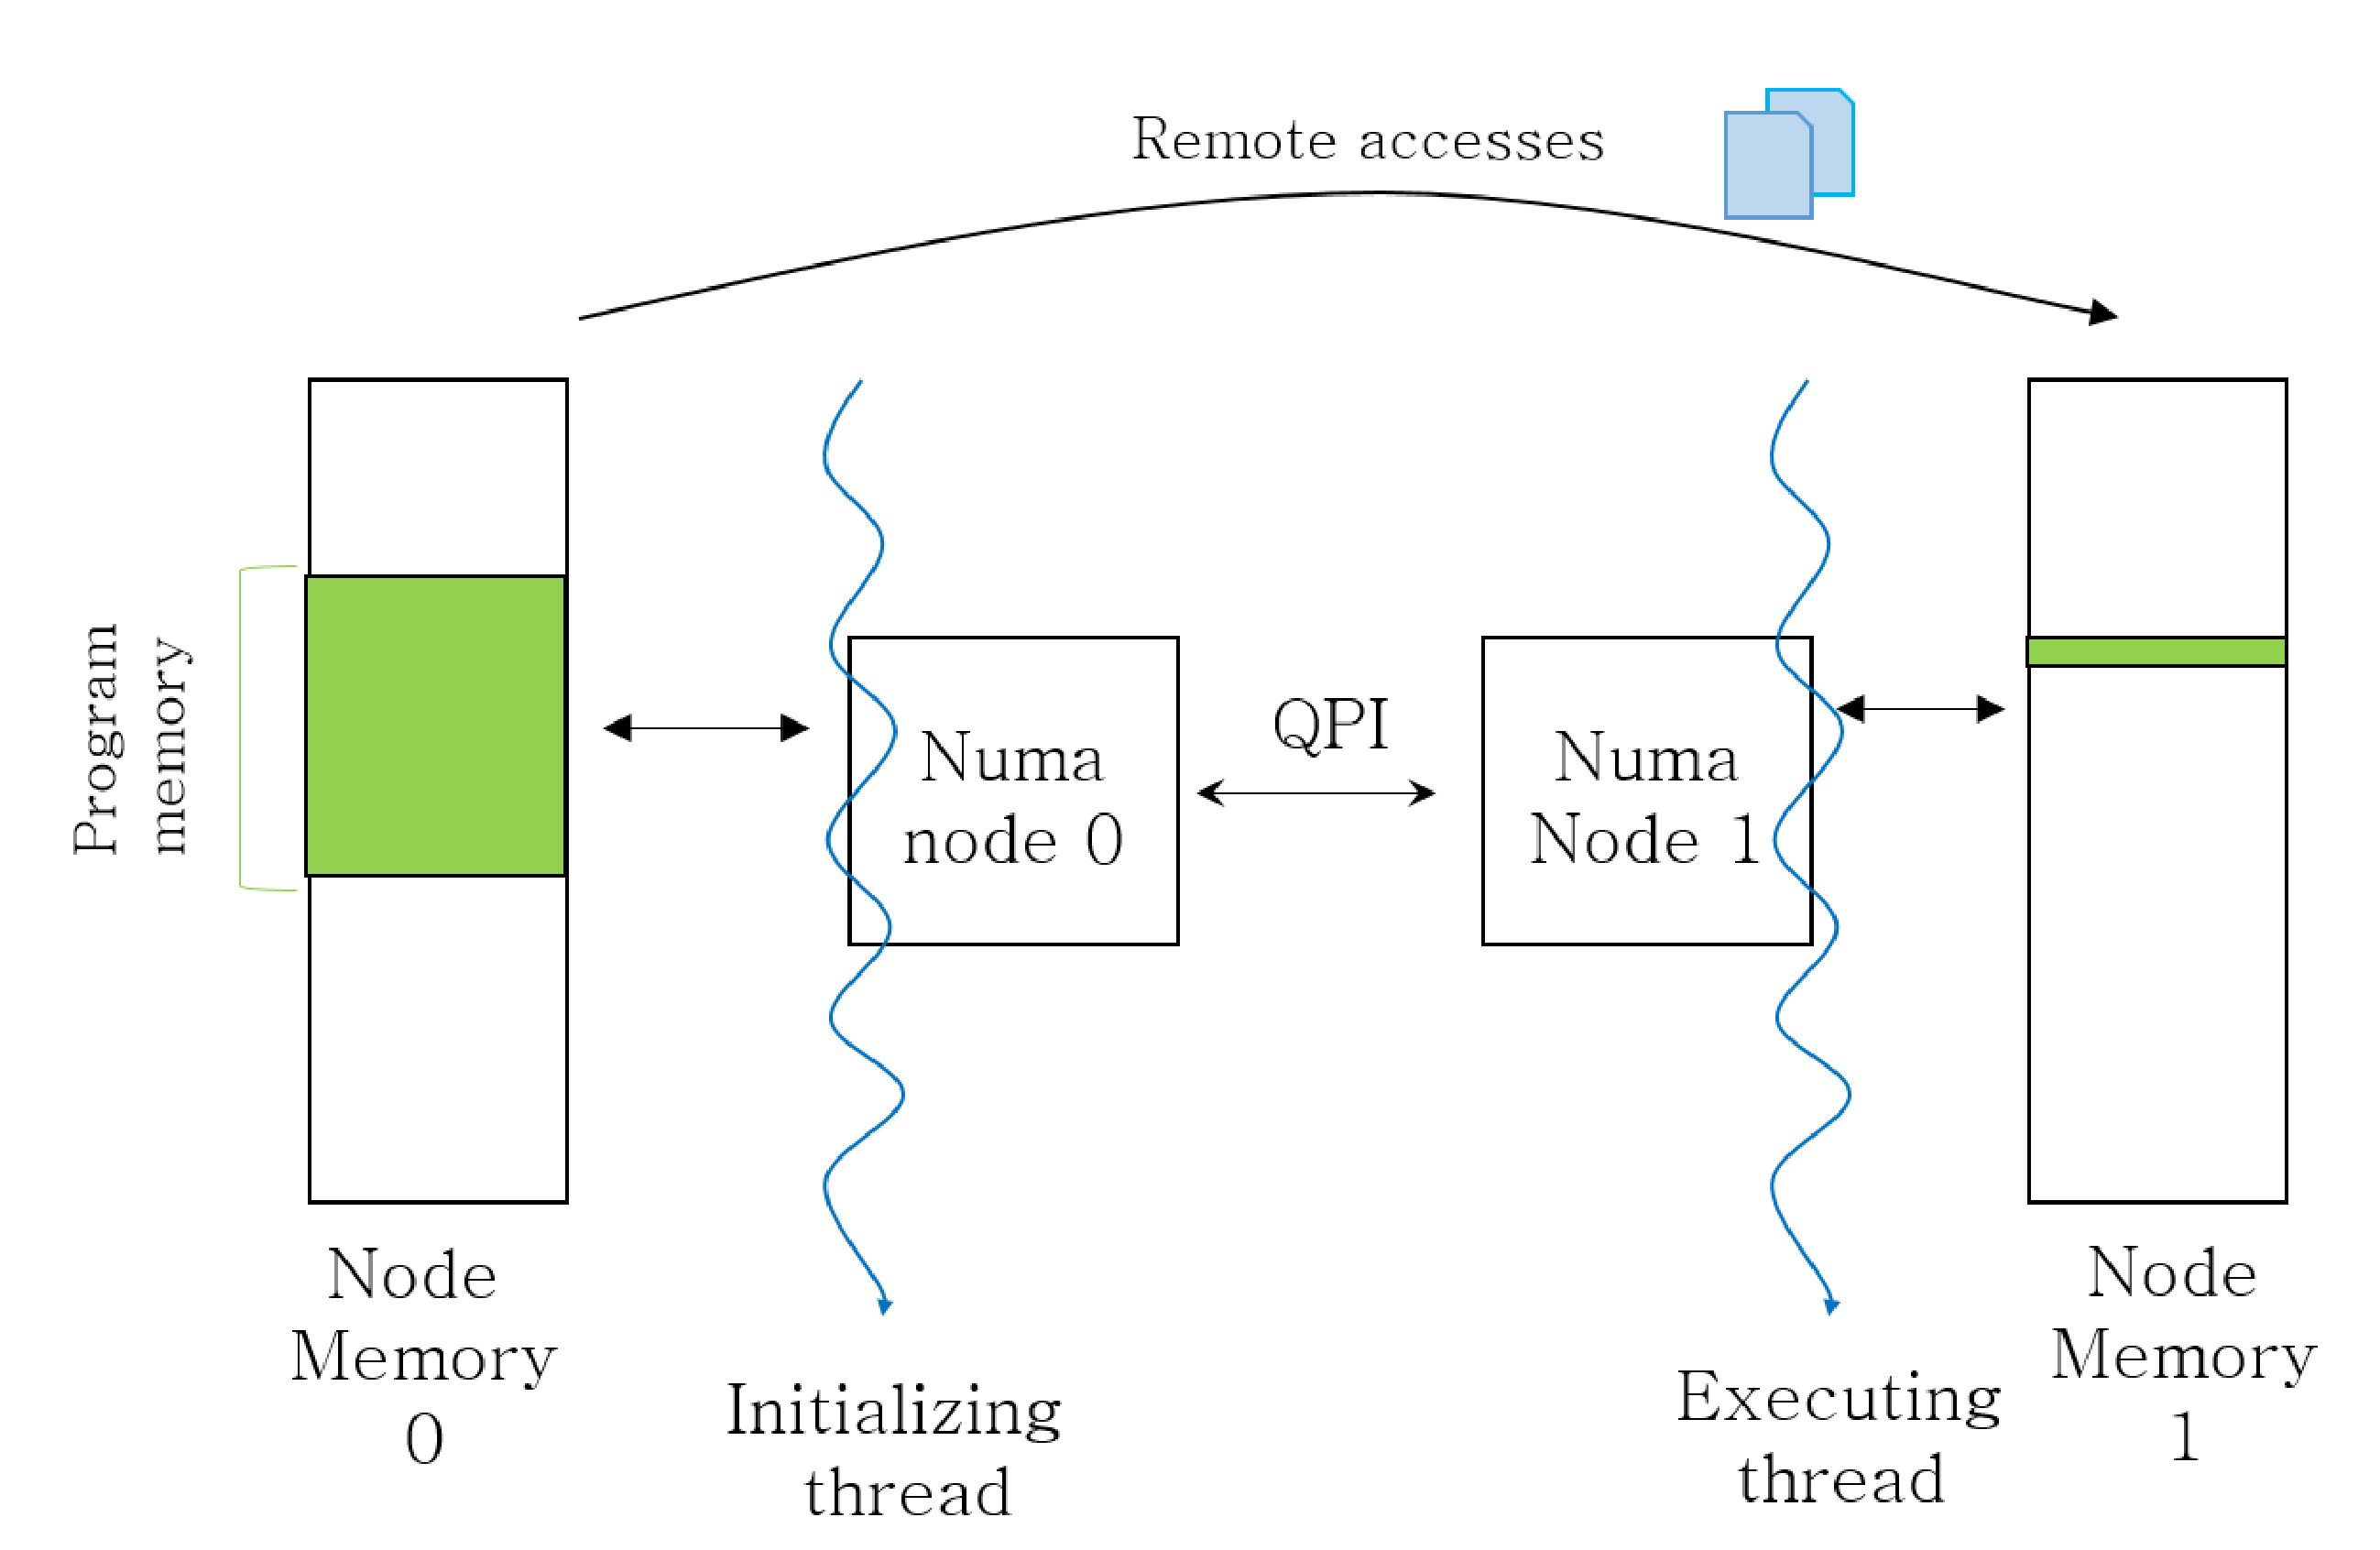
\includegraphics[width=.7\textwidth]{figures/distgentt-remote.eps}
		\caption[Depiction of the working of the distgen vanilla remote scenario with two threads]{Depiction of the distgen vanilla remote with two running threads. Each thread is pinned to a different NUMA node, which causes a lot of remote accesses to be done by the running thread.}
		\label{fig:dgentt-remote}
\end{figure}
\FloatBarrier
\subsubsection{Performance for the random mode}\label{subsection:res-dgrandom-2t-scens}

\begin{table}
	\centering
		\begin{tabularx}{\textwidth}{|l|l|l|l|X|}
		\hline
			Size & Vanilla local & Vanilla Remote & Moveall after 45s & SPM \\
			\hline
			400G & 61.470 & 102.573 & 85.375 & 80.221\\
			\hline
			600G & 91.382 & 154.340 & 124.067 & 134.695\\
			\hline
			800G & 125.757 & 215.269 & 200.078 & 187.817\\
			\hline
			1T & 151.291 & 260.406 & 198.249 & 202.729\\
			\hline
		\end{tabularx}
		\caption{Execution time given in seconds of the different distgen scenarios in random mode.}
		\label{table:res-dgentimrdm2t}
\end{table}

\begin{table}
	\centering
		\begin{tabularx}{\textwidth}{|l|l|l|l|X|}
		\hline
			Size & Vanilla local & Vanilla Remote & Moveall after 45s & SPM \\
			\hline
			400G & 1.12973E+08 & 6.77034E+07 & 1.00708E+08 & 9.68249E+07\\
			\hline
			600G & 1.13992E+08 & 6.74924E+07 & 8.24585E+07 & 9.35968E+07\\
			\hline
			800G & 1.10442E+08 & 6.45197E+07 & 7.36434E+07 & 7.10097E+07\\
			\hline
			1T & 1.14753E+08 & 6.66698E+07 & 8.85143E+07 & 9.39763E+07\\
			\hline
		\end{tabularx}
		\caption{Execution throughput given in reads per second of the different distgen scenarios in random mode.}
		\label{table:res-dgentrgrdm2t}
\end{table}

\begin{table}
	\centering
		\begin{tabularx}{.8\textwidth}{|l|l|X|}
		\hline
			Size & Moved pages & Moved pages \%  \\
			\hline
			400G & 422971 & 108.280576 \\
			\hline
			600G & 372289 & 63.53732267 \\
			\hline
			800G & 413297 & 52.902016 \\
			\hline
			1T & 423478 & 43.3641472 \\
			\hline
		\end{tabularx}
		\caption{Number of pages moved by the SPM tool for the random distgen scenario with two remote threads.}
		\label{table:res-dgenmvdrdm2t}
\end{table}


\begin{figure}[th]
	\centering
		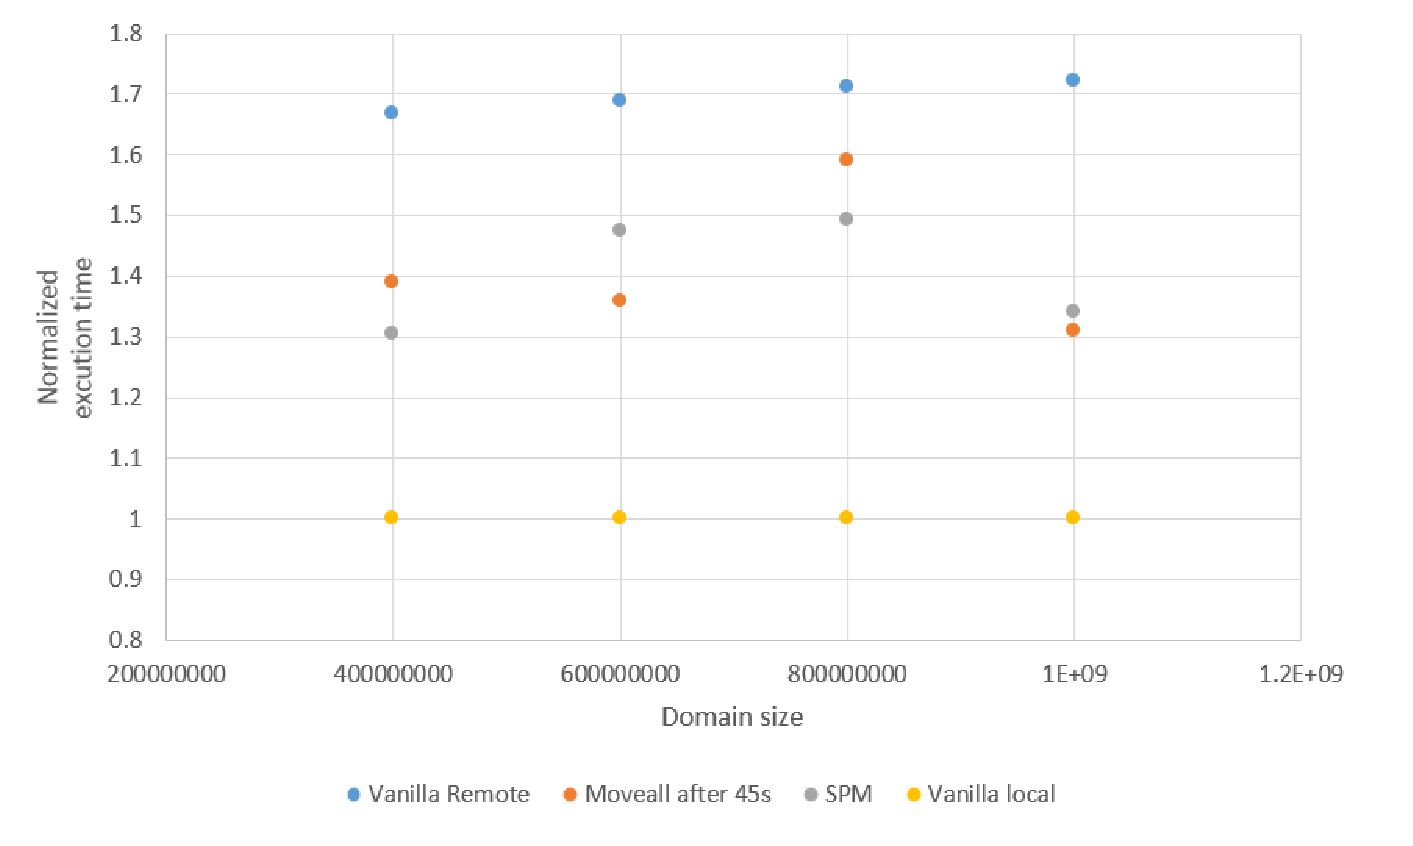
\includegraphics[width=.8\textwidth]{figures/time-dgentt-random.eps}
		\caption{Normalized execution times for the different scenarios of distgen random with two threads.}
		\label{fig:res-dgentimrdm2t}
\end{figure}

\begin{figure}[th]
	\centering
		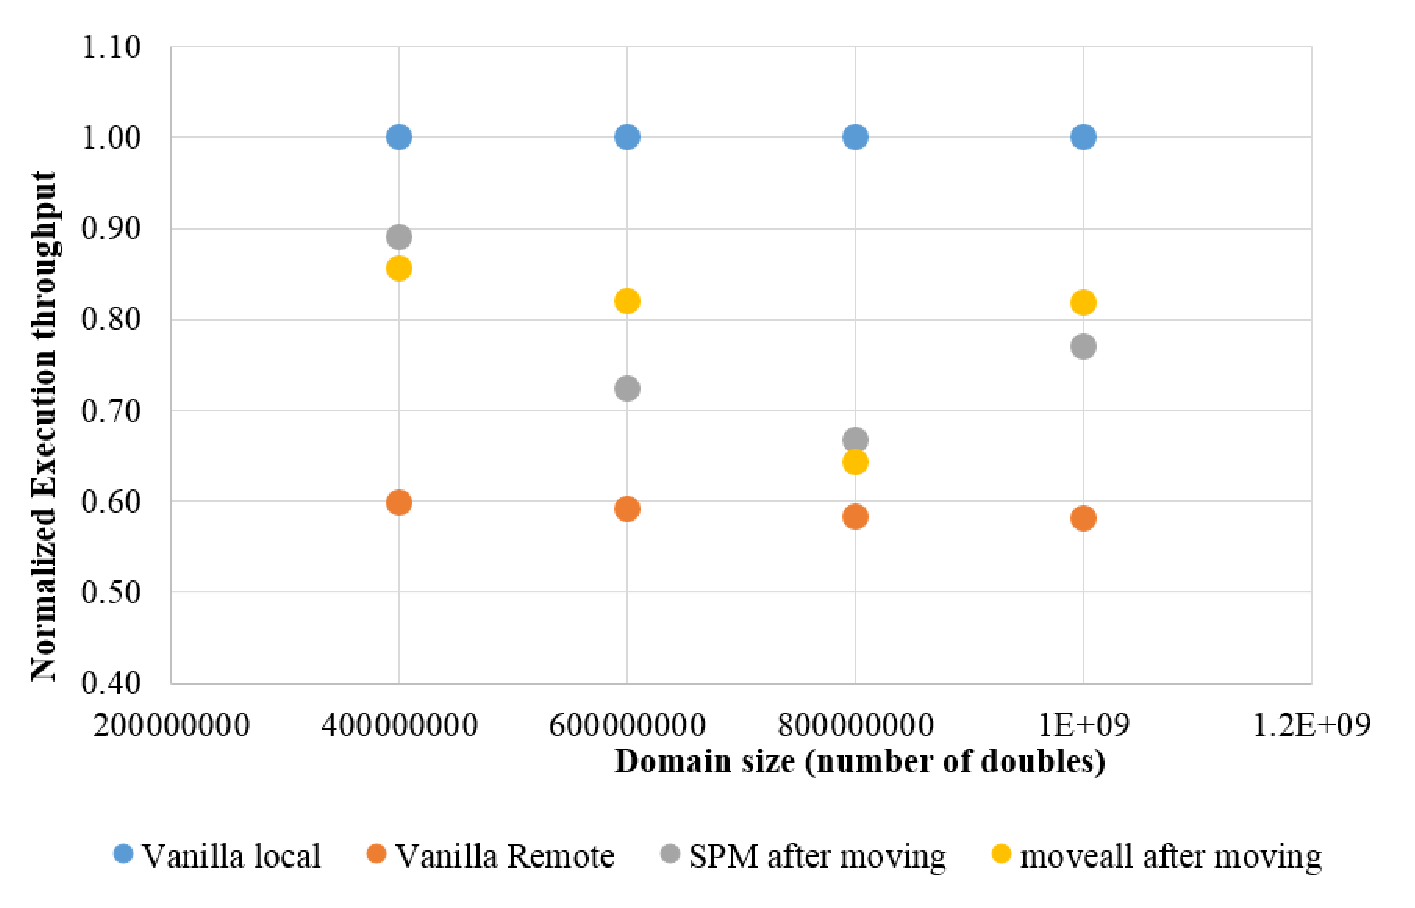
\includegraphics[width=.8\textwidth]{figures/thrput-dgentt-randm.eps}
		\caption{Normalized execution throughput for the different scenarios of distgen random with two threads}
		\label{fig:res-dgentrgrdm2t}
\end{figure}

Tables \ref{table:res-dgentimrdm2t} and \ref{table:res-dgentrgrdm2t} show the results of the execution of the different scenarios of distgen random. Figures \ref{fig:res-dgentimrdm2t} and \ref{fig:res-dgentrgrdm2t} show the execution times and throughputs respectively as a normalized quantity with respect to the distgen vanilla result, which means that a value closer to 1 resembles a performance closer to that obtained in the local algorithm. In this random setting with two threads, SPM did a very good job with a performance very similar to the moveall situation, which is the theoretical maximum that can be reached. Another important result that appears in most of the measurements, is that the performance of the moveall strategy after moving the pages never gets to be the same as that obtained in the local version, effect that has to be researched further.
As for the performance of the SPM it can be seen from table \ref{table:res-dgenmvdrdm2t} that the percentage of captured pages remain above 40 percent with decreasing value as the domain gets bigger. This happens because with a bigger domain size the observation time occupies a smaller relative portion of the total execution time and therefore less samples can be captured.

\FloatBarrier
\subsubsection{Performance for the sequential mode}\label{subsection:res-dgseq-2t}

\begin{table}[th]
	\centering
		\begin{tabularx}{\textwidth}{|l|l|l|l|X|}
		\hline
			Size & Vanilla local & Vanilla Remote & SPM & Moveall after 45s  \\
			\hline
			400G & 55.924 & 92.534  & 75.969 & 75.146\\
			\hline
			600G & 83.894 & 138.851 & 117.433 & 104.407 \\
			\hline
			800G & 111.823 & 185.144 & 159.905 & 133.699 \\
			\hline
			1T & 139.810 & 231.453 & 199.576 & 163.018 \\
			\hline
		\end{tabularx}
		\caption{Execution time for the different scenarios of the distgen sequential algorithm with units given in seconds.}
		\label{table:res-tbl-dgentimseq2t}
\end{table}

\begin{table}[th]
	\centering
		\begin{tabularx}{\textwidth}{|l|l|l|l|X|}
		\hline
			Size & Vanilla local & Vanilla Remote & Moveall after 45s & SPM \\
			\hline
			400G & 2.48368E+08 & 1.50106E+08 & 2.37636E+08& 2.37768E+08\\
			\hline
			600G & 2.48350E+08 & 1.50048E+08  & 2.37708E+08 & 1.96037E+08\\
			\hline
			800G & 2.48409E+08 & 1.50039E+08 & 2.37704E+08 & 1.86950E+08 \\
			\hline
			1T & 2.48352E+08 & 1.50023E+08 & 2.37542E+08 & 1.48624E+08 \\
			\hline
		\end{tabularx}
		\caption{Execution throughput for the different scenarios of the distgen sequential algorithm with units given in reads per second.}
		\label{table:res-dgentrgseq2t}
\end{table}

\begin{table}[th]
	\centering
		\begin{tabularx}{.6\textwidth}{|l|l|X|}
		\hline
			Size & Moved pages & Moved pages \%  \\
			\hline
			400G & 232777 & 59.590912 \\
			\hline
			600G & 234551 & 40.03003733\\
			\hline
			800G & 226748 & 29.023744 \\
			\hline
			1T & 233191 & 23.8787584 \\
			\hline
		\end{tabularx}
		\caption{Number of pages moved in the distgen sequential scenario.}
		\label{table:res-dgenmvdseq2t}
\end{table}

\begin{figure}
	\centering
		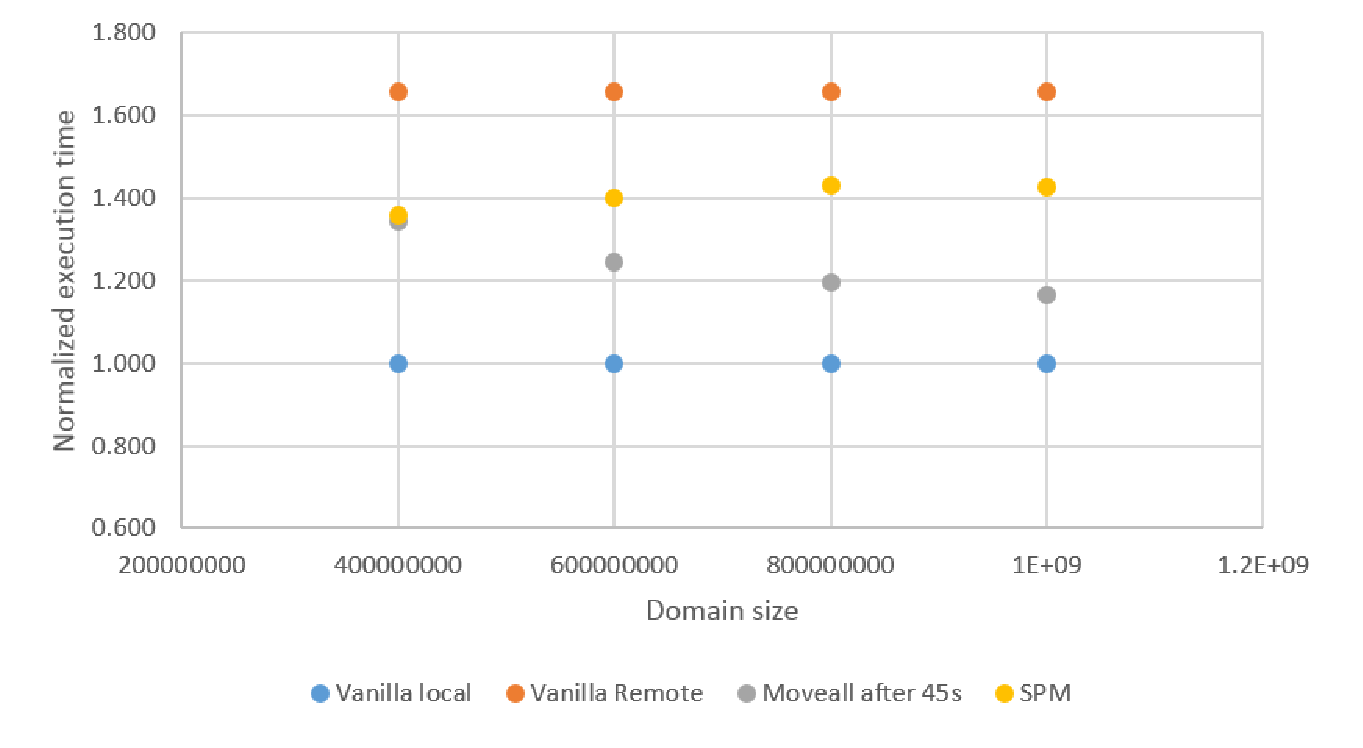
\includegraphics[width=.8\textwidth]{figures/time-dgentt-ser.eps}
		\caption{Normalized execution speed for the different scenarios of  distgen sequential with two threads with respect to the vanilla local scenario}
		\label{fig:res-dgentimseq2t}
\end{figure}

\begin{figure}
	\centering
		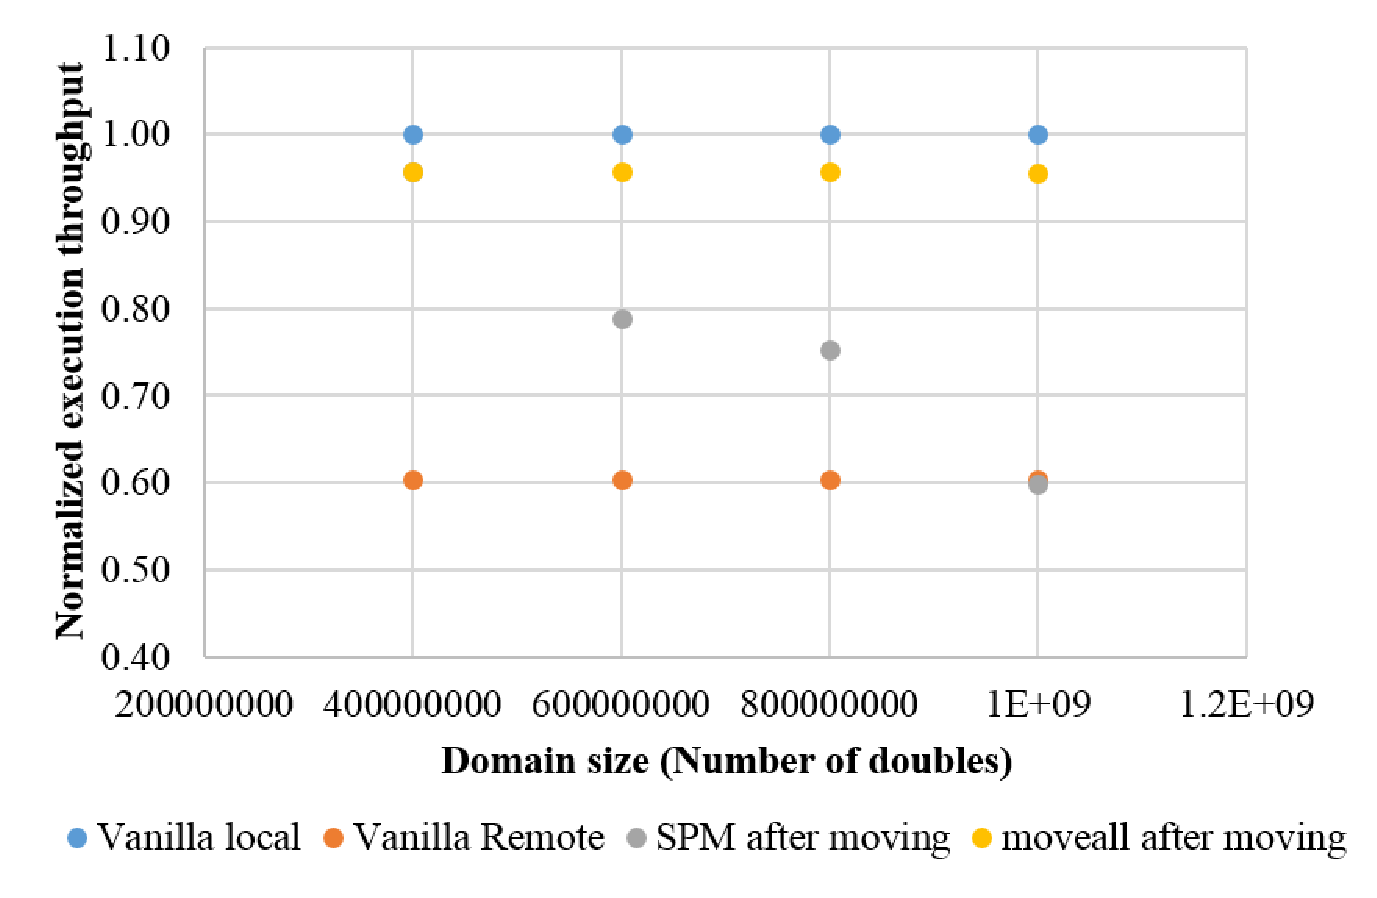
\includegraphics[width=.8\textwidth]{figures/thrput-dgentt-ser.eps}
		\caption{Normalized execution throughput for the different scenarios of the distgen sequential with two threads with respect to the vanilla local scenario.}
		\label{fig:res-dgentrgseq2t}
\end{figure}


In this opportunity the serial version of distgen is run. Because of the faster running time of this algorithm, the number of iterations is doubled to 2000 to obtain a long enough execution time that allows to observe the influence of SPM. Tables \ref{table:res-tbl-dgentimseq2t} and \ref{fig:res-dgentrgseq2t} show the execution time and performance results and Figures \ref{fig:res-dgentimseq2t} and \ref{fig:res-dgentrgseq2t} show the normalized values with respect to distgen vanilla. In comparison to the serial version the performance of the SPM tool is not as good and only matches that of the moveall scenario in with the smallest size. Part of this slowdown can be explained by the smaller portion of pages that the tool is getting, as shown in table \ref{table:res-dgenmvdseq2t}.

\subsection{SPM and distgen with all threads employed}\label{subsection:res-spmydistgen-at}

The scenarios used here follow the same logic as what was shown in the previous section, but now the goal is to go further and try a contention scenario where more cores are running the algorithm. For this test all the cores except two were used, one of the remaining ones is used to run SPM. In the remote cases, every core is mapped to a core in the opposed NUMA node and the data will be allocated in this remote node.

\subsubsection{Performance for the random mode}\label{subsection:time-dgenat-random.eps}

Table \ref{table:res-dgentimrdmat} shows the run times for the scenarios under this case and figure \ref{fig:time-dgenatt-ser} shows the normalized results. These results show that the performance of the tool locate very close to the best possible. Table \ref{table:res-tbl-dgenmvdrdmat} confirms that a good coverage of the computing domain was reached.

Table \ref{table:res-dgentimserat} shows the completion time information and figure \ref{fig:time-dgenatt-ser} shows these quantities normalized. Unlike the random case the improvement is not so good, locating itself between the worst and possible cases. Table \ref{table:res-tbl-dgenmvdseqat} could point to a possible cause to be the lowest coverage of the computing domain obtained.

\begin{table}[th]
	\centering
		\begin{tabularx}{\textwidth}{|l|l|l|l|X|}
		\hline
			Size & Vanilla local & Vanilla Remote & Moveall after 45s & SPM \\
			\hline
			90G & 83.51 & 196.688 & 152.959 & 155.405\\
			\hline
			110G & 103.617 & 242.471 & 184.673 & 191.259\\
			\hline
			130G & 129.617 & 282.619 &194.029 & 210.215\\
			\hline
			150G & 141.588 & 329.403 & 260.219 & 254.283\\
			\hline
		\end{tabularx}
		\caption{Completion time in seconds for the random distgen with 30 threads employed}
		\label{table:res-dgentimrdmat}
\end{table}

\begin{figure}[th]
	\centering
		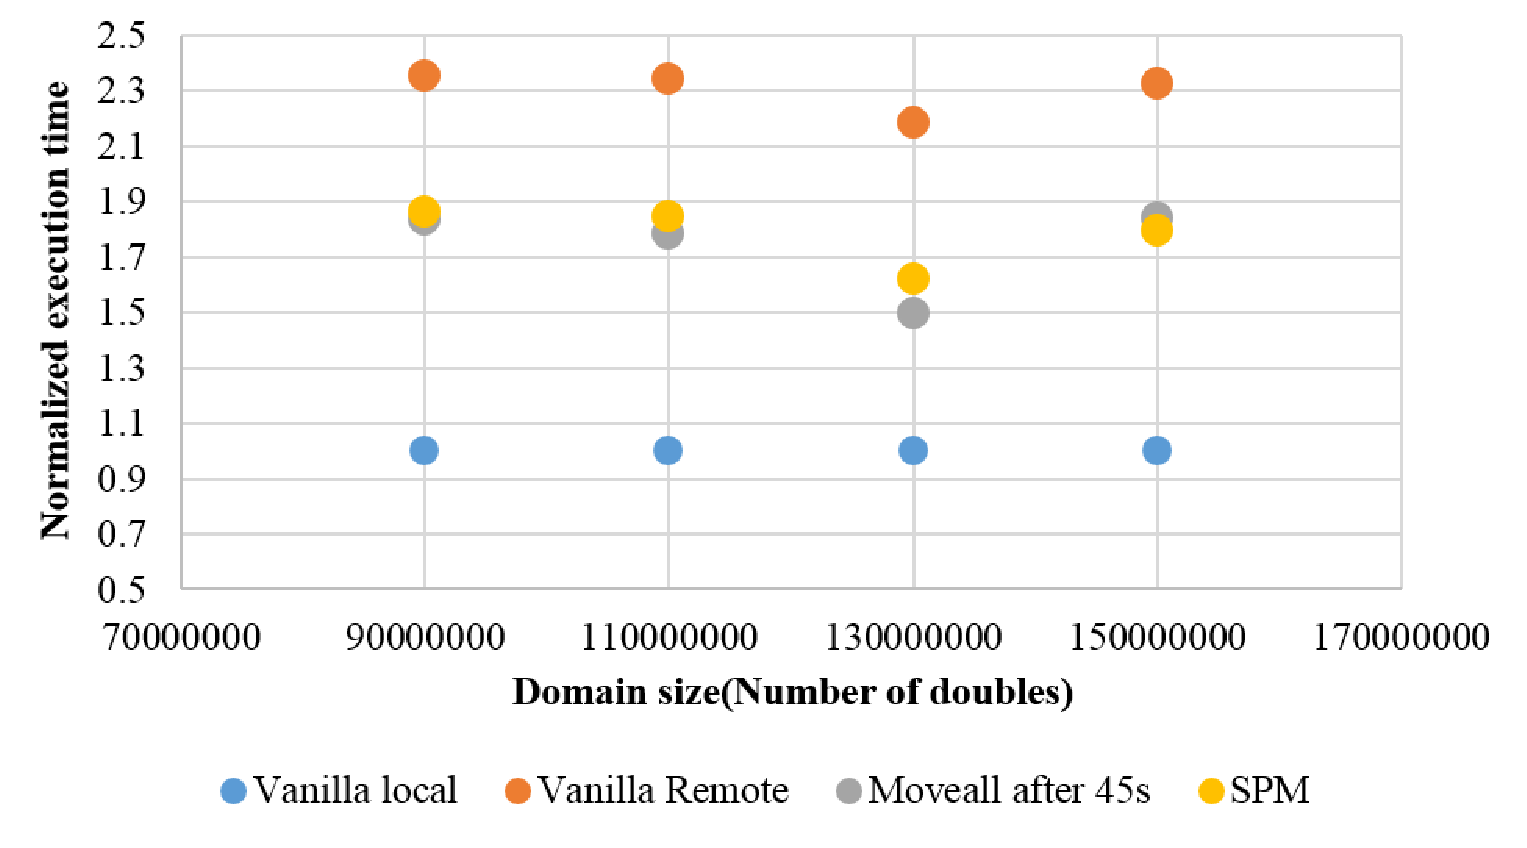
\includegraphics[width=.8\textwidth]{figures/time-dgenat-random.eps}
		\caption{Normalized execution time for the random distgen cases with 30 threads employed.}
		\label{fig:res-dgentimrdmat}
\end{figure}



\subsubsection{Performance for the sequential mode}\label{subsection:time-dgenat-seq.eps}

\begin{table}[th]
	\centering
		\begin{tabularx}{\textwidth}{|l|l|l|l|X|}
		\hline
			Size & Vanilla local & Vanilla Remote & Moveall after 45s & SPM \\
			\hline
			90G & 127.763 & 341.35 & 152.959 & 262.535\\
			\hline
			110G & 156.145 & 417.683 & 184.673 & 331.794\\
			\hline
			130G & 184.482 & 493.134 & 194.029 & 395.134\\
			\hline
			150G & 212.992 & 569.438 & 260.219 & 465.617\\
			\hline
		\end{tabularx}
		\caption{Normalized execution time for the sequential distgen cases with 30 threads employed.}
		\label{table:res-dgentimserat}
\end{table}

\begin{figure}[th]
	\centering
		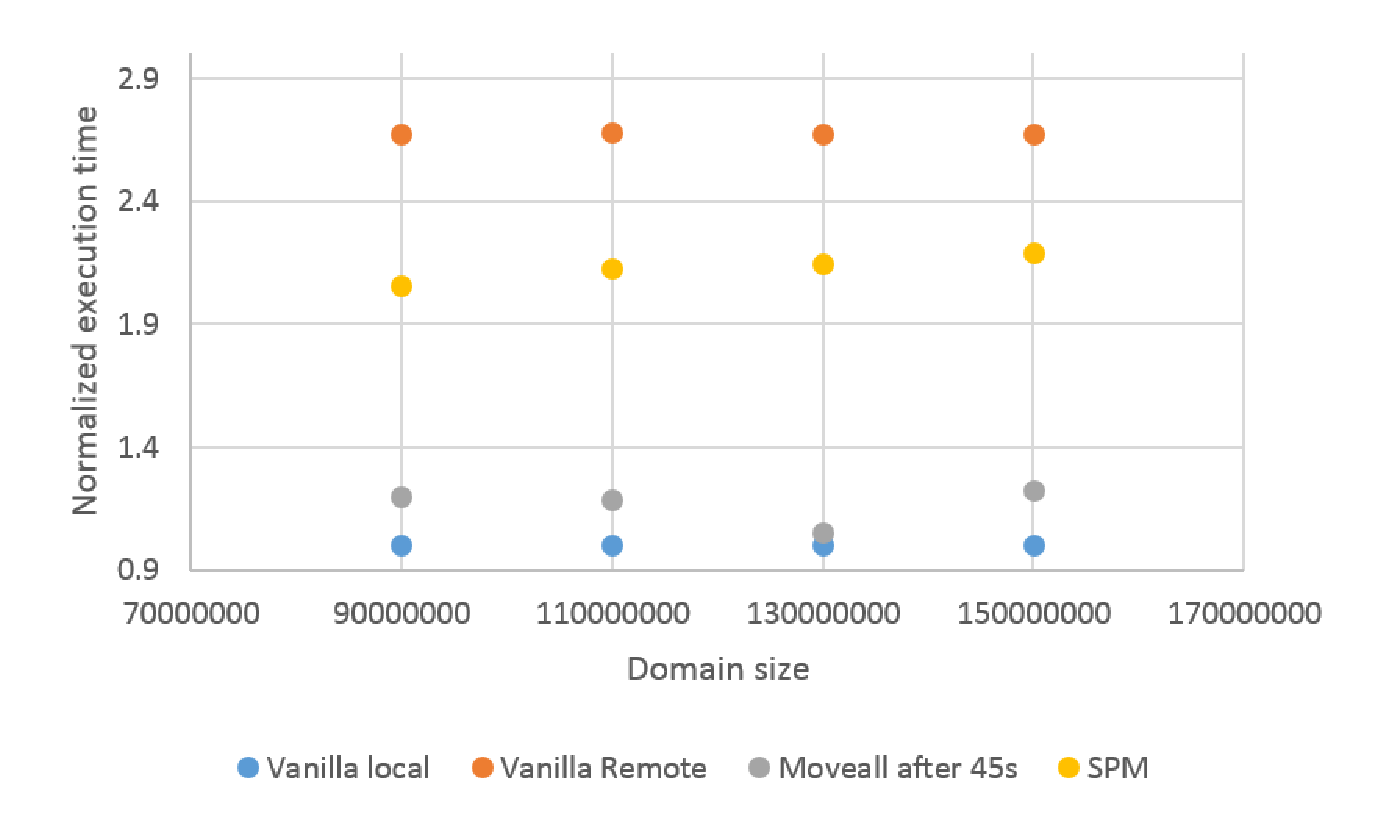
\includegraphics[width=.8\textwidth]{figures/time-dgenatt-ser.eps}
		\caption{Normalized execution time for the sequential distgen cases with 30 threads employed.}
		\label{fig:time-dgenatt-ser}
\end{figure}

\begin{table}[th]
	\centering
		\begin{tabularx}{.6\textwidth}{|c|c|c}
		\hline
			Size & Moved pages & Moved pages \%  \\
			\hline
			90G & 4438270 & 84.16274963 \\
			\hline
			110G & 4556914 & 54.38554704 \\
			\hline
			130G & 3526065 & 46.29090462 \\
			\hline
			150 & 4647763 & 52.88121458 \\
			\hline
		\end{tabularx}
		\caption{Number of moved pages by the SPM tool for the distgen random case with 30 active threads.}
		\label{table:res-tbl-dgenmvdrdmat}
\end{table}


\begin{table}[th]
	\centering
		\begin{tabularx}{.6\textwidth}{|l|l|X|}
		\hline
			Size & Moved pages & Moved pages \%  \\
			\hline
			90G & 770653 & 13.70049778 \\
			\hline
			110G & 809007 & 11.76737455 \\
			\hline
			130G & 809901 & 9.96801230 \\
			\hline
			150 & 853033 & 9.099018667 \\
			\hline
		\end{tabularx}
		\caption{Number of moved pages by the SPM tool for the distgen sequential case with all threads engaged.}
		\label{table:res-tbl-dgenmvdseqat}
\end{table}
\FloatBarrier
\subsubsection{Measuring the effect of SPM's action}\label{subsection:time-dgenat-action.eps}

\begin{figure}[th]
	\centering
		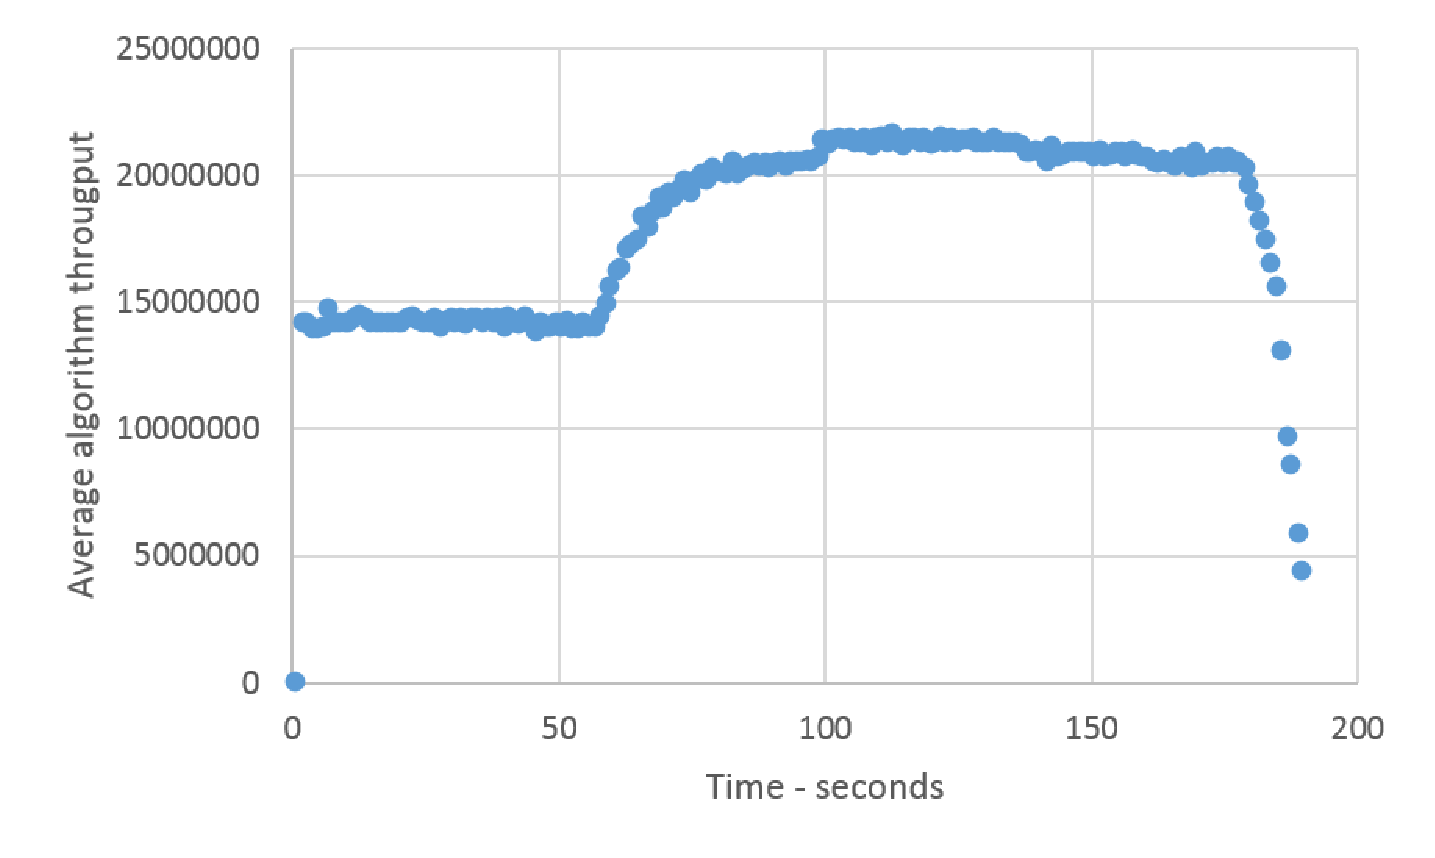
\includegraphics[width=.8\textwidth]{figures/at-thrput-random.eps}
		\caption{View of the average throughput during the execution of distgen under SPM supervision in the distgen spm case with 30 active threads and a domain of size 110G. The page migration is done at time 45.}
		\label{fig:at-spmactn-thgput}
\end{figure}

\begin{figure}[th]
	\centering
		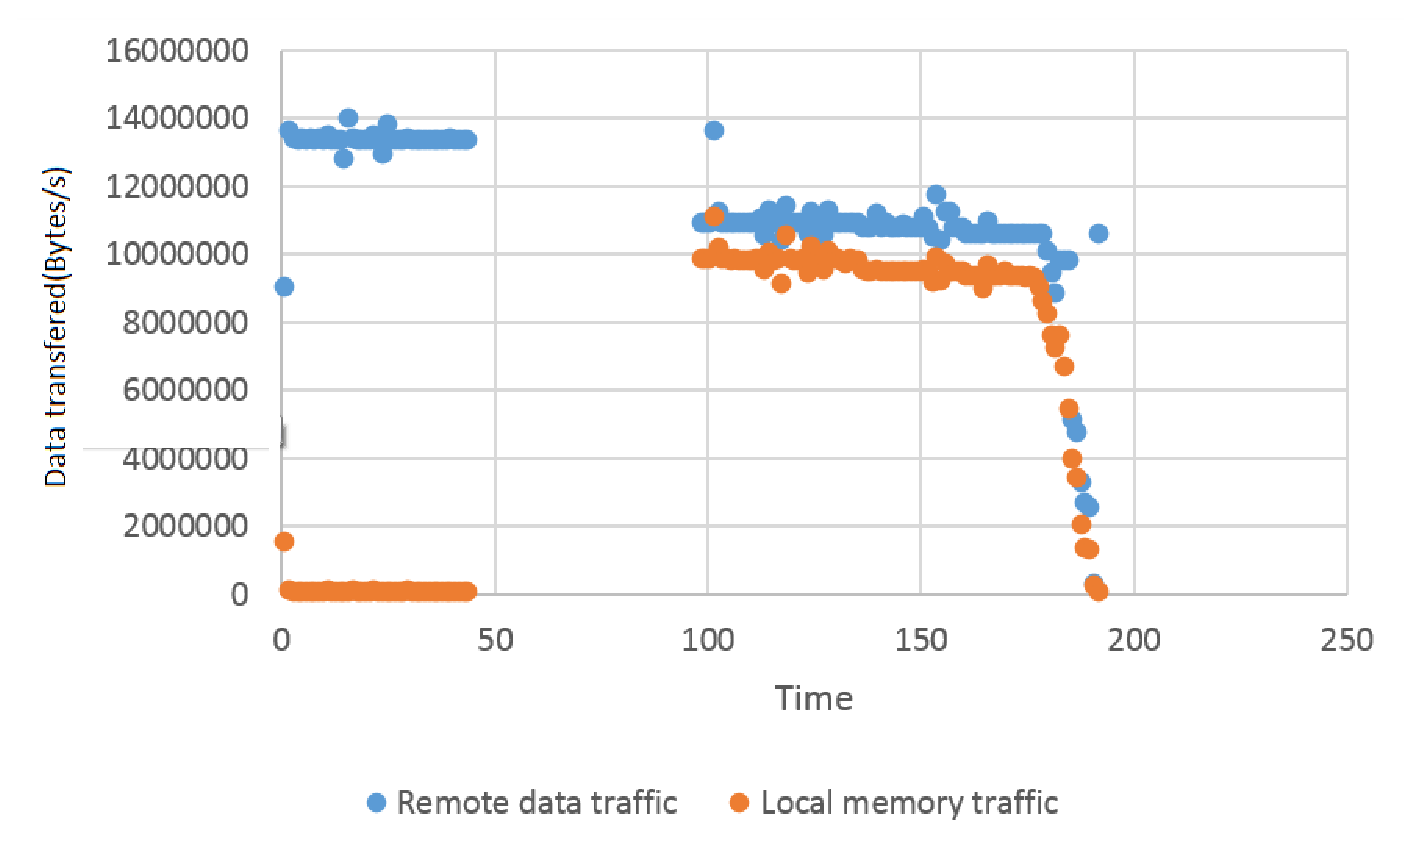
\includegraphics[width=.8\textwidth]{figures/at-transfer-random.eps}
		\caption{View of the average and local and remote transfer rates during the execution of distgen under SPM supervision in the distgen spm case with 30 active threads and a domain of size 110G. The page migration is done at time 45.}
		\label{fig:at-spmactn-trsfer}
\end{figure}

A more detailed way to appreciate the improvements in performance of the SPM is to look at the information provided by the performance readings: the first one is the average number of executed instructions, which is shown in figure \ref{fig:at-spmactn-thgput} as a function of time. After the end of the observation period there are more instructions executed. 

The second way to verify the action of SPM is to look at the performances average values of local and remote memory traffic, which are shown in figure \ref{fig:at-spmactn-trsfer}. After the end of the observation phase, the local traffic increases and the remote decreases working in favor of a more efficient execution of the observed algorithm.

\section{SPM and LAMA-CG}\label{section:spmylamacg}

For the execution of LAMA-CG a contention situation with 30 threads will be used to test the action of SPM, leaving one for the execution of the SPM tool. This time the source code of the observed algorithm will not be modified, but in order to create a situation with many remote accesses involved, the re-pinning of the threads was be induced 15 seconds after starting the algorithm in such a way that every thread was reallocated to a core located in the opposite NUMA node and then SPM was started as usual.

For the study of LAMA-CG under SPM a variation of parameters was done by trying sampling periods of 10, 20 and 50 instructions per sample and observation phase times of 60 and 120 seconds. Three domain sizes were used, which were square matrices of length 3000, 3750 and 4500.


\begin{table}
	\centering
		\begin{tabularx}{\textwidth}{|l|l|l|l|l|X|}
		\hline
			Size & Original & Flipped & Flipped SPM & Flipped SPM  & Flipped SPM \\
			 &  &  no-SPM & c=10  &c=20 &c=50\\
			\hline
			3000 & 166 & 250 & 189 & 221 & 233\\
			\hline
			3750 & 308 & 509 & 350 & 443 & 465\\
			\hline
			4500 & 532 & 915 & 577 & 750 & 770\\
			\hline
		\end{tabularx}
		\caption{Run times for the Lama-cg scenarios with a measurement time of 60 seconds}
		\label{table:lamatim60}
\end{table}

\begin{table}
	\centering
		\begin{tabularx}{\textwidth}{|l|l|l|l|l|X|}
		\hline
			Size & Original & Flipped & Flipped SPM & Flipped SPM  & Flipped SPM \\
			 &  &  no-SPM & c=10  &c=20 &c=50\\
			\hline
			3000 & 166 & 250 & 234 & 228 & 237\\
			\hline
			3750 & 308 & 509 & 465 & 484 & 481\\
			\hline
			4500 & 532 & 915 & 746 & 824 & 823\\
			\hline
		\end{tabularx}
		\caption{Run times for the Lama-cg scenarios with a measurement time of 120 seconds}
		\label{table:lamatim120}
\end{table}
\begin{figure}[th]
	\centering
		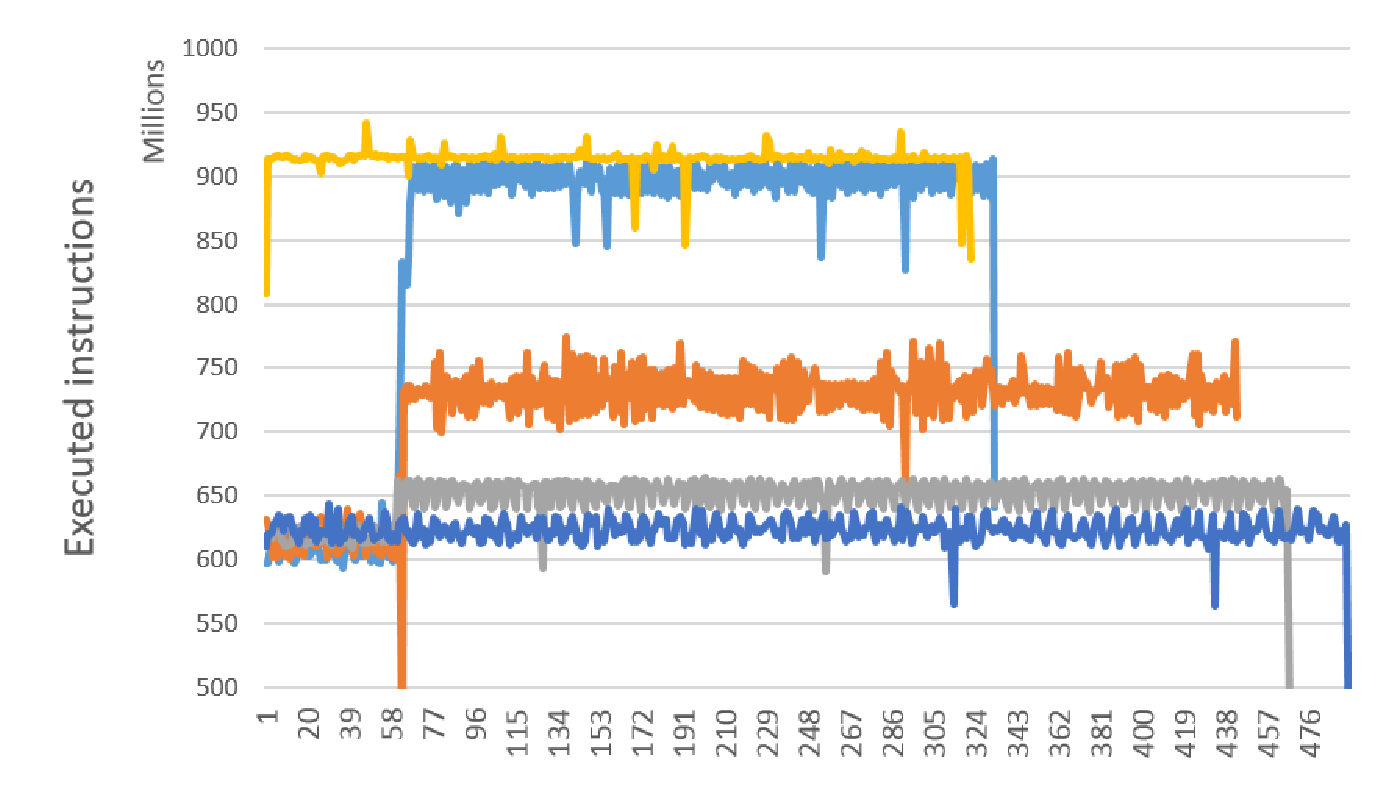
\includegraphics[width=\textwidth]{figures/lama-thrput.eps}
		\caption{Average executed instructions as a function of time for the executions of LAMA-CG with measurement time of 60 seconds and matrix size of 3750.}
		\label{fig:res-lamatrg}
\end{figure}

\begin{figure}[th]
	\centering
		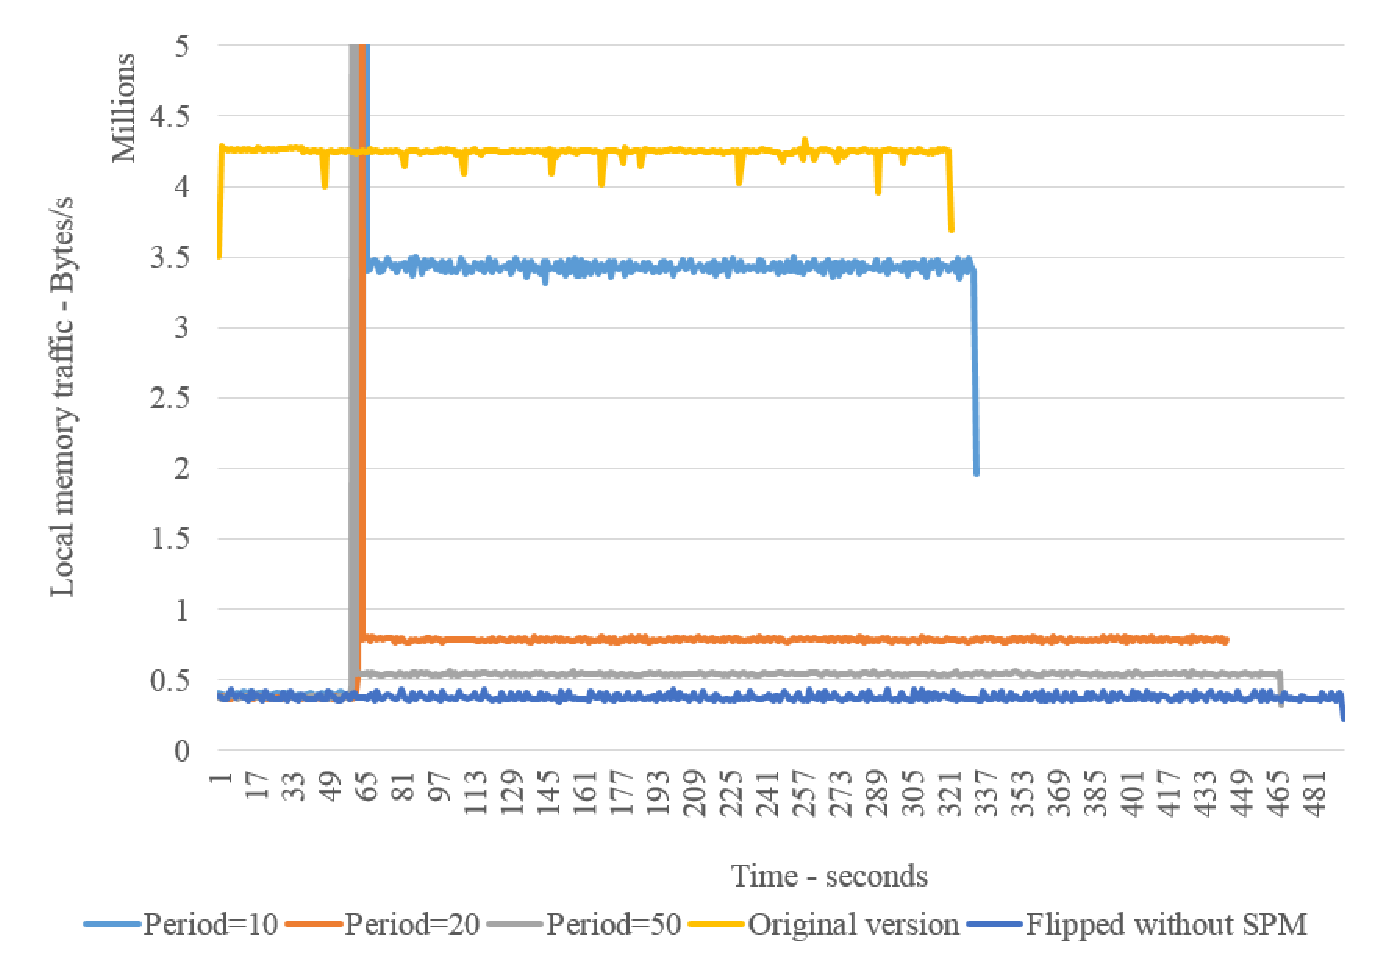
\includegraphics[width=.9\textwidth]{figures/lama-localtr.eps}
		\caption{Average local memory traffic as a function of time for the executions of LAMA-CG with measurement time of 60 seconds and matrix size of 3750.}
		\label{fig:res-lamaloctr}
\end{figure}

Tables \ref{table:lamatim60} and \ref{table:lamatim120} show the run time results for the different scenarios described above. The results show that the best times are obtained with the lowest period of 10 instructions per sample. The biggest observation time was only best for the biggest size.

Figure \ref{fig:res-lamatrg} shows the throughput readings for the different scenarios of the matrix with size 3750 and observation time of 60 seconds: the original version is the best case with the highest throughput and the flipped version is the worst case because a lot of remote accesses are performed. The other three cases show the intervention of the SPM tool after 60 seconds of re-pinning the threads. The readings for local memory and remote memory transfers are shown in figures \ref{fig:res-lamatrg} and \ref{fig:res-lamatrg} respectively.

\begin{figure}[th]
	\centering
		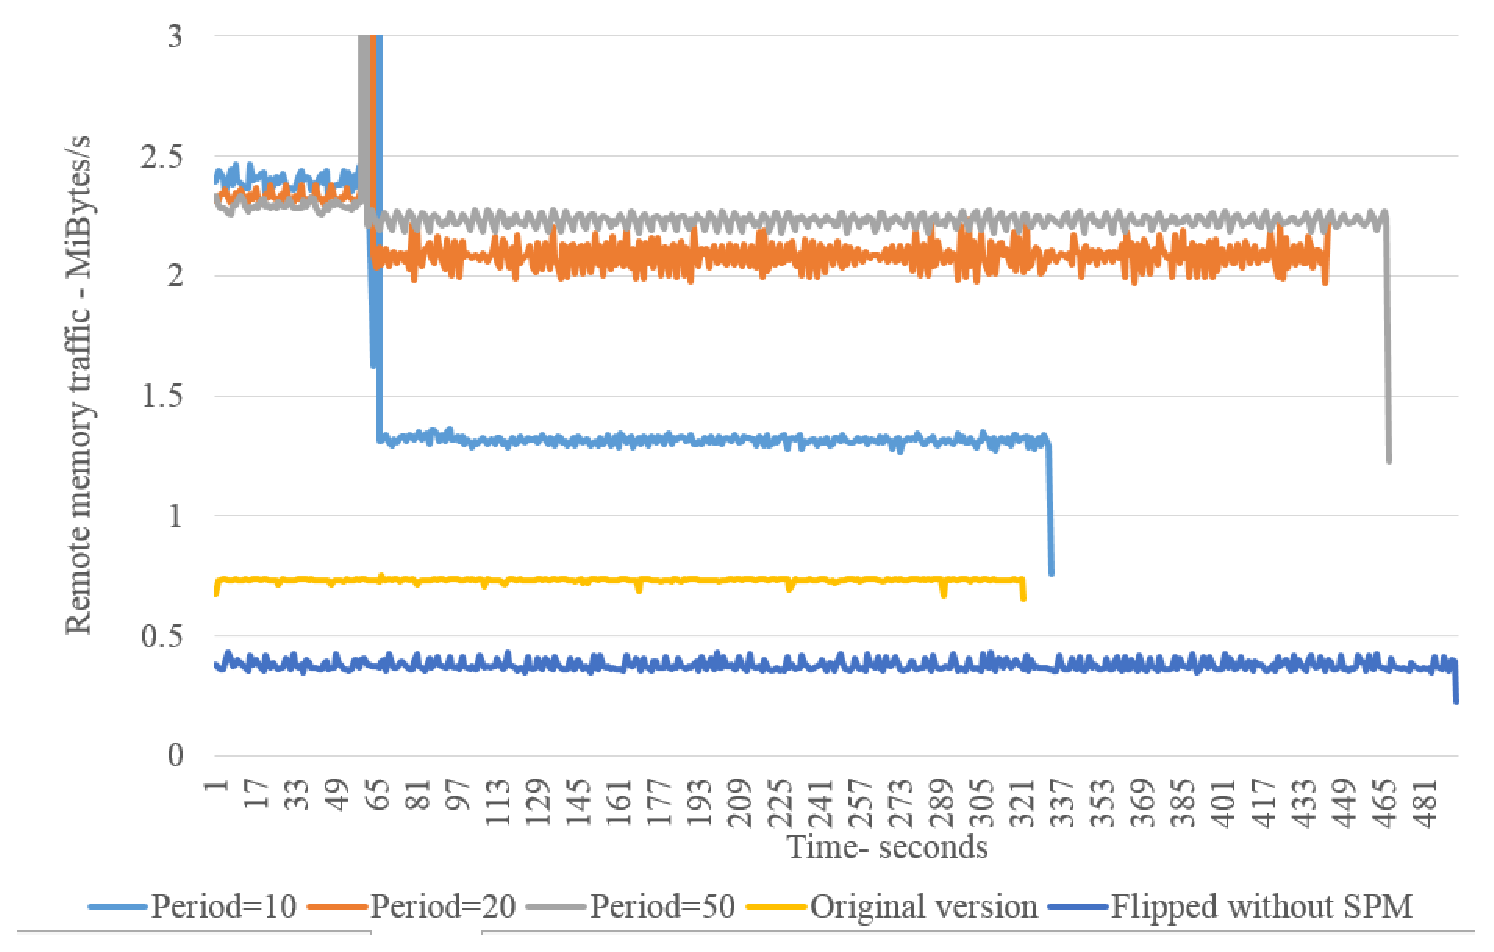
\includegraphics[width=.9\textwidth]{figures/lama-remotetr.eps}
		\caption{Average remote memory traffic as a function of time for the executions of LAMA-CG with measurement time of 60 seconds and matrix size of 3750.}
		\label{fig:res-lamaremotr}
\end{figure}